\documentclass[a4paper]{article}
\usepackage[italian]{babel}

% immagini
\usepackage{graphicx}
\usepackage{svg}

% matematica
\usepackage{amsmath}
\usepackage{amsfonts}

% codice
\usepackage{listings}
\lstset{
    basicstyle=\small\ttfamily,
    numbers=left,
    numberstyle=\small\ttfamily
}

\usepackage{blindtext}
\usepackage{titlesec}
\usepackage{geometry}
\usepackage{relsize}
\usepackage{tikz}
% \geometry{
% a4paper,
% total={190mm,257mm},
% left=25mm,
% right=25mm,
% top=50mm,
% }


\sloppy % ?

\begin{document}

\begin{titlepage} % pagina riservata al titolo
    \begin{center}
        \vspace*{1cm}
        {\Huge\bfseries Analisi di algoritmi di selezione\par}
        \vspace{.5cm}
        {\LARGE Progetto di laboratorio di Algoritmi e Strutture Dati\par}
        \vspace{1cm}
        \begin{figure}[h]
            \centering
            
\includegraphics[width=.5\textwidth]{uniud_logo.pdf}
        \end{figure}
        \vspace{1.5cm}
        {\LARGE Università degli studi di Udine\par}
        {\LARGE Dipartimento di scienze Informatiche, Matematiche e Fisiche\par}
        \vfill
        {\Large Anno Accademico 2023/2024\par}
        {\Large Matricole: 162367, 162473\par}
        {\Large\itshape Gerardi Ludovico, Sclauzero Lorenzo, Pantanali Riccardo\par}
    \end{center}
\end{titlepage}
\newpage
\section{Introduzione}
Il progetto ha come scopo l'implementazione ed analizzare la complessità di tre algoritmi di selezione. Che calcolano il k-esimo elemento più piccolo di un vettore non ordinato di interi.\\
L'analisi dell'efficienza dei tre algoritmi viene effettuata attraverso la misurazione dei tempi medi\\
I tre algoritmi discussi all'interno della relazione per la risoluzione del problema prendono il nome di $Quick\ Select$, $Heap\ Select$ e $Medians\ of\ Medians$: come si vedrà nei prossimi paragrafi, le diverse procedure adottano dei metodi molto diversi questa differenza di approcci vengono riflesse nei grafici.\\
\section{Presentazione degli Algoritmi}
\subsection{Algoritmi calcolo k-esimo elemento}
\textbf{Quick Select}\ La procedura in ogni chiamata ricorsiva su un intervallo $[i,j]$
 del vettore fornito in input termina restituendo il $k-esimo$ elemento più piccolo del vettore qualora $k-1\in[i,j]$, oppure un valore indefinito qualora k$\not\in[i,j]$. L'algoritmo ha una complessità asintotica di $\Theta(n^2)$
 nel caso pessimo e $O(n)$ nel caso medio, dove $n$ è il numero di elementi del 
 \vspace{2mm}
 vettore.\\
\textbf{Heap Select}\ Questo algoritmo di selezione utilizza due min$-$heap, denominate H1 e H2. La prima heap H1 é costruita a partire dal vettore fornito in input in tempo lineare e non viene modificata.
La seconda heap \( H2 \) contiene inizialmente un solo nodo, corrispondente alla radice di \( H1 \). All'i-esima iterazione, per \( i \) che va da 1 a \( k-1 \), l'algoritmo estrae la radice di \( H2 \), che corrisponde a un nodo \( x_i \) in \( H1 \), e reinserisce in \( H2 \) i nodi successori (figli sinistro e destro) di \( x_i \) nella heap \( H1 \). Dopo \( k-1 \) iterazioni, la radice di \( H2 \) corrisponderà al \( k-esimo \) elemento più piccolo del vettore fornito in input.
L'algoritmo descritto ha complessità temporale $O(n+klogk)$\\
\vspace{2mm}
sia nel caso pessimo che in quello medio.\\\textbf{Medians of Medians}\ L'algoritmo descritto è un algoritmo basato sulla suddivisione di un vettore in blocchi di dimensione limitata (5 elementi), il calcolo della mediana di ciascun blocco e il calcolo della mediana delle mediane dei blocchi stessi. Questa mediana viene utilizzata per partizionare l'array attorno ad essa, similmente alla procedura "partition" dell'algoritmo "quick sort". A seconda del valore \( k \) fornito in input, l'algoritmo esegue chiamate ricorsive sulla parte sinistra o destra dell'array rispetto alla mediana calcolata. 

Sono proposti tre diversi approcci:
\begin{enumerate}
    \item Ricorsivo: Che alloca un nuovo vettore ad ogni chiamata ricorsiva per memorizzare le mediane dei blocchi.
    \item Quasi in place: Riutilizza lo spazio allocato per il vettore originariamente fornito in input.
    \item In place: Privo di chiamate ricorsive e riutilizza lo spazio del vettore originario.
\end{enumerate}
In tutti i casi, la complessità temporale e spaziale dell'algoritmo nel caso pessimo è \( O(n) \).
\\
\section{Misurazione dei tempi di esecuzione}
La misurazione dei tempi necessari per calcolare il k-esimo numero in un array viene effettuata considerando la lunghezza \( n \) dell'array di input e l'errore massimo consentito. Per ogni lunghezza dell'array, gli algoritmi implementati ripetono il calcolo del k-esimo numero un numero di volte tale da garantire un errore massimo relativo pari a \( f_{\max} = 0.001 \), assicurando così un tempo totale maggiore o uguale a \( T_{\min} \), calcolato come \[ T_{\min} = R \left( \frac{1}{f} + 1 \right) \] dove \( R \) rappresenta la risoluzione del clock.

Ciascuna iterazione del calcolo del k-esimo numero viene eseguita su un array generato pseudo-casualmente di lunghezza \( n \), differente ad ogni iterazione.
\newpage
\section{Rappresentazione grafica dei risultati}
\subsection{Caso k costante}
\begin{figure}[h]
            \centering
            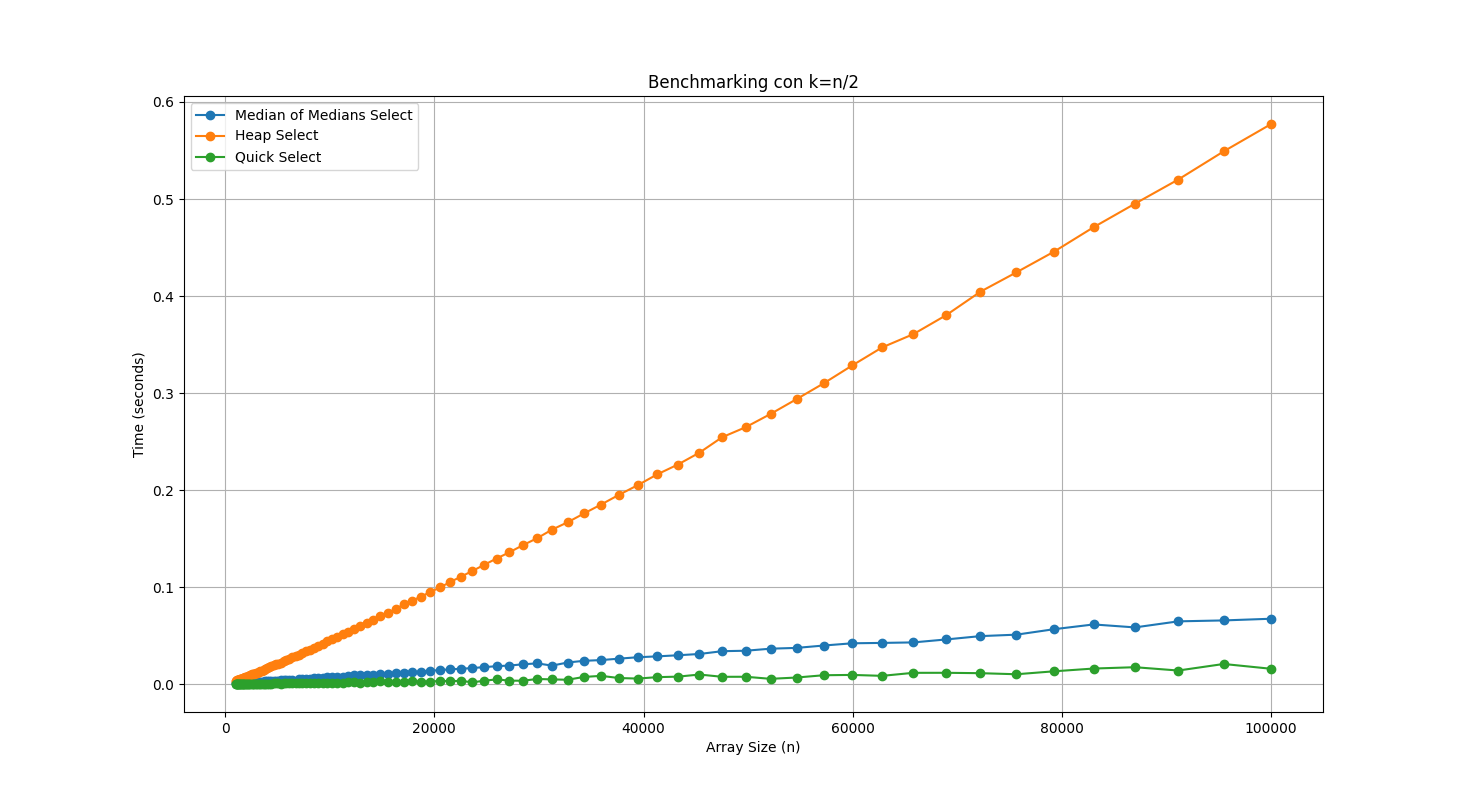
\includegraphics[width=.83\textwidth]{graphs/K_const_n.png}
            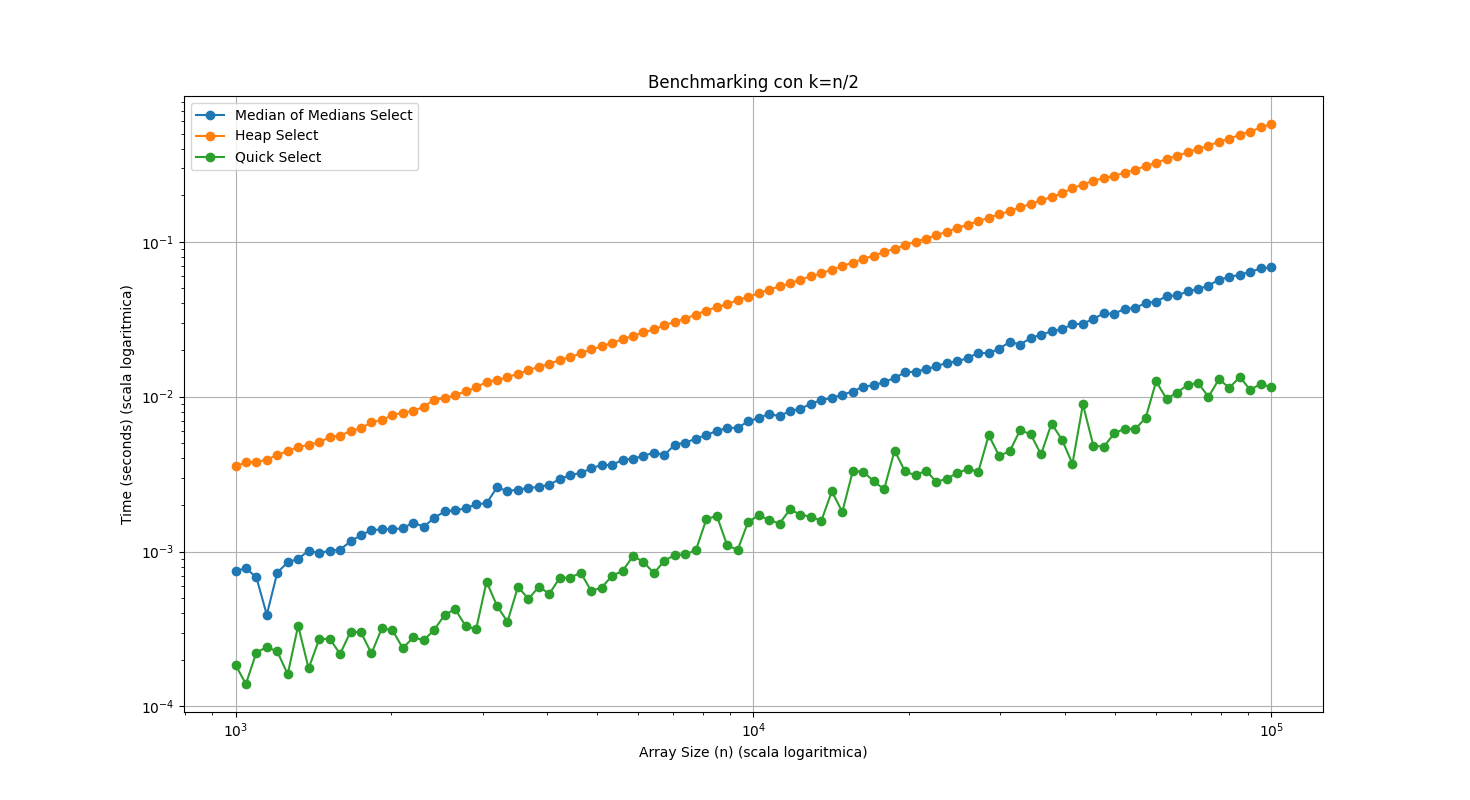
\includegraphics[width=.83\textwidth]{graphs/K_const_2xlog.png}
\end{figure}
\newpage
\begin{figure}[h]
            \centering
            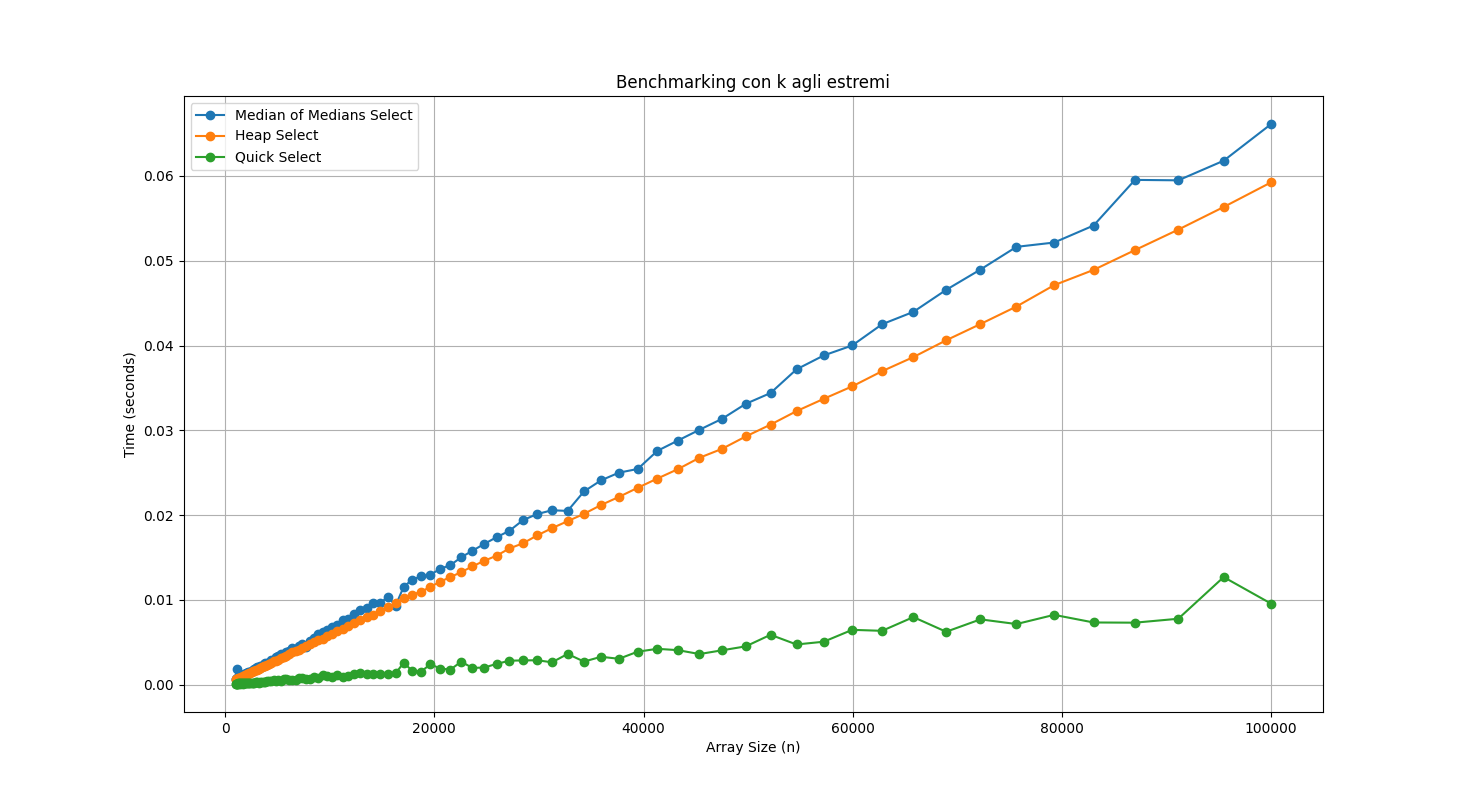
\includegraphics[width=.83\textwidth]{graphs/K_last_n.png}
            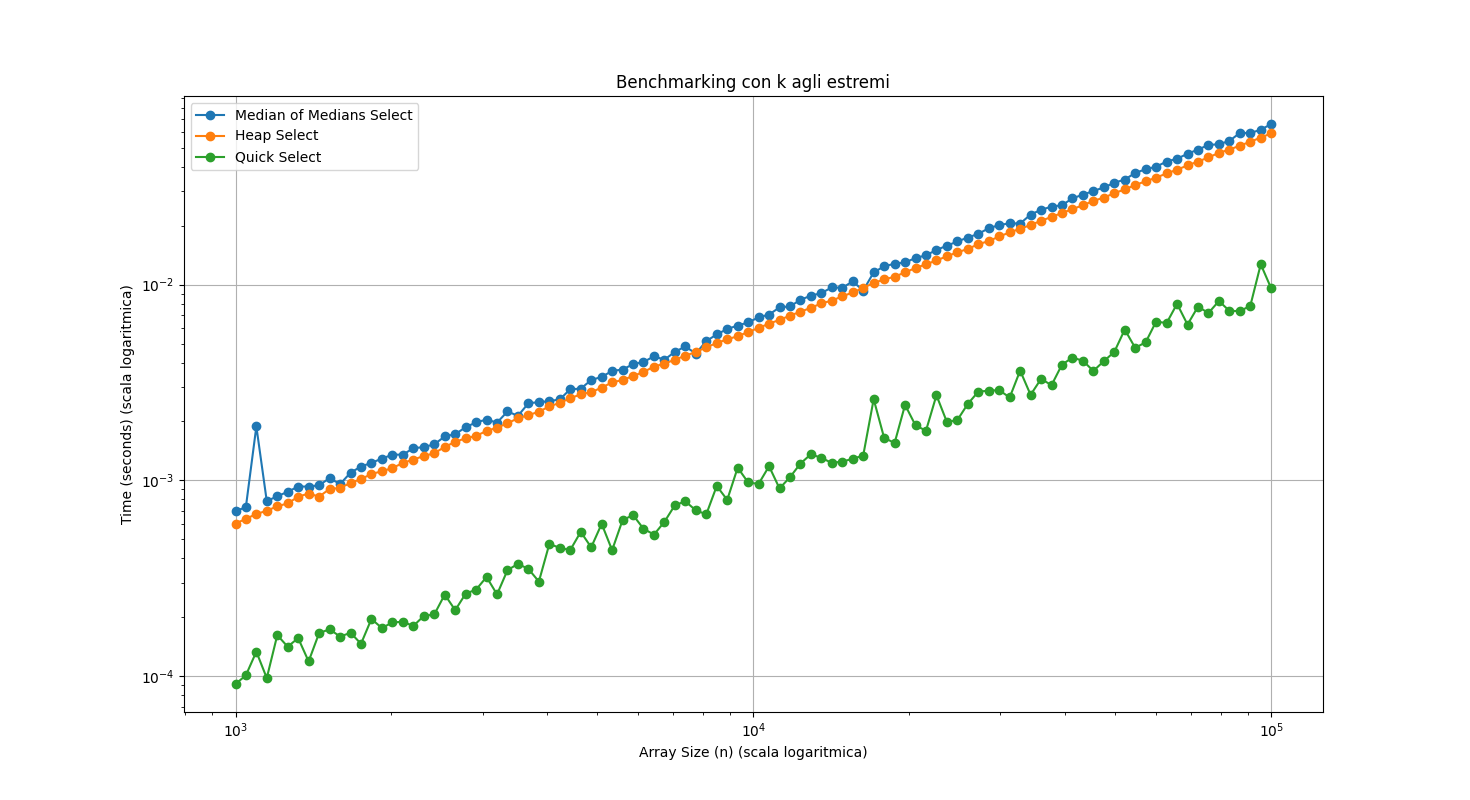
\includegraphics[width=.83\textwidth]{graphs/K_last_2xlog.png}
\end{figure}
\newpage
\subsection{Caso k random}
\begin{figure}[h]
            \centering
            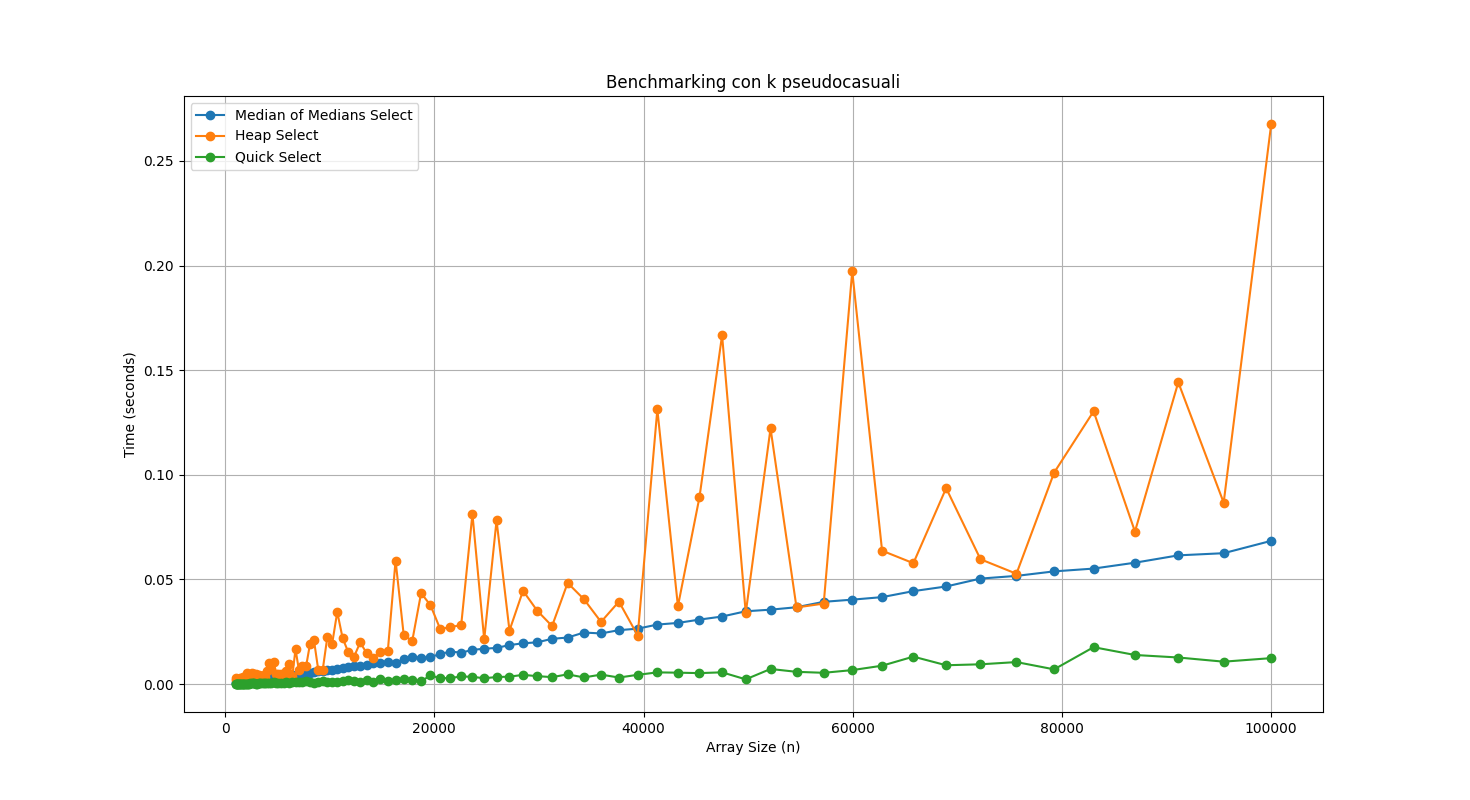
\includegraphics[width=.83\textwidth]{graphs/K_random_n.png}
            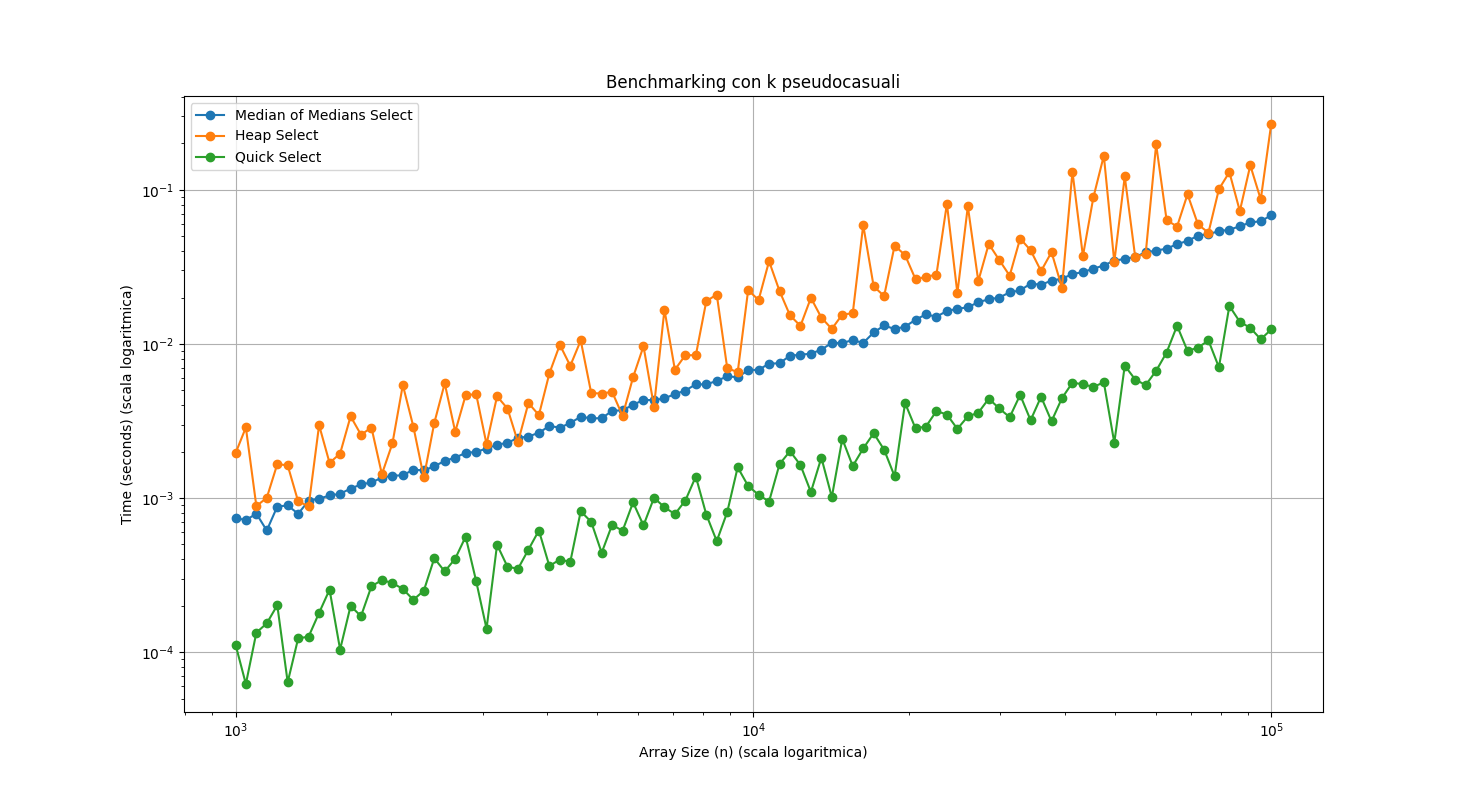
\includegraphics[width=.83\textwidth]{graphs/K_random_2xlog.png}
\end{figure}
\end{document}